\chapter{Bluetooth Low Energy}
\label{ch:ble}
%http://www.medicalelectronicsdesign.com/article/bluetooth-low-energy-vs-classic-bluetooth-choose-best-wireless-technology-your-application
%http://www.link-labs.com/bluetooth-vs-bluetooth-low-energy/
%http://www.quora.com/Is-there-a-difference-between-Bluetooth-4-0-and-Bluetooth-Low-Energy-If-so-what


\section{Definition}
\gls{bleLabel} (auch \textit{Bluetooth Smart} genannt) ist eine optionale Erweiterung zum klassischen Bluetooth 4.0.
Dabei wurde besonders Wert auf einen stromsparenden Betrieb und eine günstige Herstellung der Chips gelegt, wobei eine deutlich geringere Übertragungsrate in Kauf genommen werden muss.

Da die Spezifikation von \gls{bleLabel} lediglich auf Softwaredefinitionen beruht, können sämtliche Bluetooth Geräte mit einem \textit{Firmware Upgrade} die Unterstützung anbieten.

Das Einsatzgebiet von \gls{bleLabel} richtet sich besonders an Geräte, die regelmässig kleine Datenmengen übertragen sollen.
Der Stromverbrauch ist so gering, dass ein Gerät mit einer gewöhnlichen Knopfzellenbatterie mehrere Jahre betrieben werden kann. Konkret kann eine Übertragungsrate von maximal 1\,MBit/s (resp. von 0.271\,MBit/s Nutzdaten) bei einem maximalen Stromverbrauch von 15\,mA erreicht werden.
Falls keine Daten übermittelt werden, wird der \gls{bleLabel} Chip in einen Sleep-Modus versetzt, indem er nur noch $1\,\si{\micro A}$ benötigt.

\gls{bleLabel} kann in zwei verschiedenen Modi implementiert werden:\footcite{Bluetooth_Low_Energy_vs_Classic_Bluetooth_Medical_Electronics_Design_2015-04-27}
\begin{itemize}
	\item \textbf{Single-Modus:} Geräte im Single-Modus ("`Smart Devices"') unterstützen einzig \gls{bleLabel} und sind auf einen geringen Stromverbrauch optimiert.
	\item \textbf{Dual-Modus:} Geräte im Dual-Modus ("`Smart Ready Devices"') unterstützen klassisches Bluetooth, wie auch \gls{bleLabel}. Dadurch das beide Technologien angeboten werden, verliert sich der Vorteil des geringen Stromverbrauches, wie auch der Kostenvorteil. Dieser Modus ist typisch für Computers und Smartphones.
\end{itemize}


\subsection{Geschichte}
Nokia erkannte im Jahr 2001 das Bedürfnis einer stromsparenden und kabellosen Übertragungsmöglichkeit. Resultierend wurde 2004 \textit{Bluetooth Low End Extension} veröffentlicht.
Zwei Jahre später und mit Hilfe anderen Firmen, wurde 2006 das Produkt \textit{Wibree} präsentiert.
Bereits 2007 wurde mit der \gls{sigLabel} eine Integration von Wibree in den Bluetooth Standard verhandelt, der 2010 in der Bluetooth Version 4.0 als \gls{bleLabel} implementiert wurde.

Das \textit{iPhone 4s} unterstützte mit \textit{iOS 5} (Juni 2011) als erstes Smartphone \gls{bleLabel}.
Darauf folgten \textit{Linux 3.4} (Mai 2012), \textit{Windows 8} (Mai 2012), \textit{Blackberry 10} (Januar 2013), \textit{Android 4.3} (Juli 2013) und schlussendlich auch \textit{Windows Phone 8.1} (April 2014).
\footcite{Bluetooth_low_energy_Wikipedia_2015-04-17}


\section{Unterschiede zu klassischem Bluetooth}
Die Unterschiede zwischen klassischem Bluetooth und \gls{bleLabel} sind sehr übersichtlich auf Wikipedia aufgelistet.\footcite{Bluetooth_low_energy_Wikipedia_2015-04-17}
Die Informationen wurden mit folgenden konkreten technischen Spezifikationen zweier aktuellen Chips von Texas Instruments ergänzt:
\textit{CC2564 Bluetooth and Dual-Mode Controller}\footcite{CC2564_DualMode_2015-05-08} und \textit{CC2541 SimpleLink Bluetooth Smart and Proprietary Wireless MCU}.\footcite{CC2541_BLE_2015-05-08}

Zusätzlich sind verschiedene Arbeiten von effektiven Messungen verfügbar, wie z.B. von Texas Instruments. \footcite{powerconsumption_comparison_2015-04-27}

Folgend eine verkürzte Liste mit den interessantesten Verschiedenheiten:
\begin{table}[H]
	% style
	\small\sffamily\renewcommand{\arraystretch}{1.4}
	% caption
	\captionabove{Vergleich: \gls{bleLabel} und klassisches Bluetooth}
	\begin{tabular}{p{0.35\linewidth}lp{0.35\linewidth}}
		\toprule
		Spezifikation & Klassisches Bluetooth & \gls{bleLabel}\\
		\midrule
		Theoretischer Datendurchsatz & 1 -- 3\,MBits/s & 1\,MBits/s (auch mit 2\,MBits/s)\\
		Effektiver Datendurchsatz (Appliaction) & 0.7 -- 2.1\,Mbit/s	& 0.27\,Mbit/s\\
%		Leistung & 1\,W & 0.01 -- 0.5\,W\\
		
		Stromverbrauch (Standby) & 1 -- 40\,$\si{\micro A}$ &  0.4 -- 1.0 \,$\si{\micro A}$ \\
		Stromverbrauch (Empfangen) & 39 -- 62\,mA &  5.9 -- 17.9\,mA \\
		
%		Max. Stromverbrauch & 30\,mA & 15\,mA\\
%		Durchschnittlicher Stromverbrauch & MISSING VALUE & 1 -- 15\,mA \\
		Verbindungszeit & 100\,ms & 6\,ms (bereits nach 0.5\,ms möglich)\\
		Übertragungszeit & 100\,ms & 3\,ms\\
		Kosten & ab 2.14\,\$ & ab 1.79\,\$ \\
		Audioübertragung & unterstützt & nicht möglich\\
		\bottomrule
	\end{tabular}
\end{table}
%http://www.argenox.com/bluetooth-low-energy-ble-v4-0-development/library/a-guide-to-selecting-a-bluetooth-chipset/
% Stromverbrauch (sleep: 1µA; active 1-15mA)

%\footcite{Bluetooth_Bluetooth_Low_Energy_Products_TIcom_2015-05-08}

\section{Kommunikation}
Um bei \gls{bleLabel} die Energie-Effizienz zu erhalten, wird der Chip so oft wie möglich in den Sleepmode gesetzt. Daten werden also nur über kurze Zeiten (stromintensiv) verschickt und empfangen, anschliessend wird in den Stromsparmodus gewechselt.
Eine Sendung dauert zwischen 7.5\,ms und 16\,s.
Sollen mehr Daten ausgetauscht werden, so kann die Verbindung über ein Reconnect verlängert werden.
\footcite[][5]{ti_whitepaper_2015-05-08}

% Dadurch, dass sich bei \gls{bleLabel} jeder Channel über 2 MHz erstreckt, reduziert sich ...

% The channel spacing of Bluetooth low energy is 2 MHz in contrast to BR’s 1 MHz, this has the effect of reducing demands on RF filtering.
% Moving up a bit, Bluetooth low energy connections are essentially similar to BR’s so-called sniff sub-rating mode.
% This provides Bluetooth low en- ergy with an energy-efficient way of maintaining connections while keeping the radio off as much as possible. Not immediately apparent from the Bluetooth specifications is the fact that the relaxed requirements allow IC vendors to do a lot of optimizations that are difficult or impossible to make with “classic” Bluetooth, lowering sleep and active currents and shortening switching times. These optimizations enable single-mode chips to be lower power, simpler and lower cost than dual-mode or classic chips.

% The minimum supported period in Bluetooth low energy is 7.5 ms, the maximum is 16 seconds. The 16 second limit is related to a communications time-out; if longer times are needed, it is possible to drop the connection and then reconnect every time as needed.

\subsection{Verbindungsaufbau}
\label{subsec:bleConnectionSetup}
Der Verbindungsaufbau von \gls{bleLabel} unterscheidet sich vom klassischen Bluetooth (siehe \cref{sec:connectionSetup}).

Anstatt den 79 Channels, gibt es bei \gls{bleLabel} nur 37 Channels. Während beim klassischen Bluetooth die Clients auf 32 verschiedenen Channels gesucht werden, wird bei \gls{bleLabel} die Suche nur auf drei Channels durchgeführt.
Dadurch dass nur ein Zehntel der Channels abgesucht wird, ergibt sich ein massiver Zeitvorteil was sich natürlich auch auf den Stromverbrauch auswirkt.\footcite[][3]{ti_whitepaper_2015-05-08}


\subsection{Protokoll Architektur}
Ein wesentlicher Vorteil von \gls{bleLabel} besteht darin, dass alle Profile auf dem \gls{gattLabel} Protokoll basieren.
Dies schränkt zwar die Flexibilität gegenüber dem klassischen Bluetooth ein, vereinfacht aber die Komplexität und reduziert die Menge an Code um einzelne Profile zu unterstützen.
\begin{figure}[H]
	\centering
	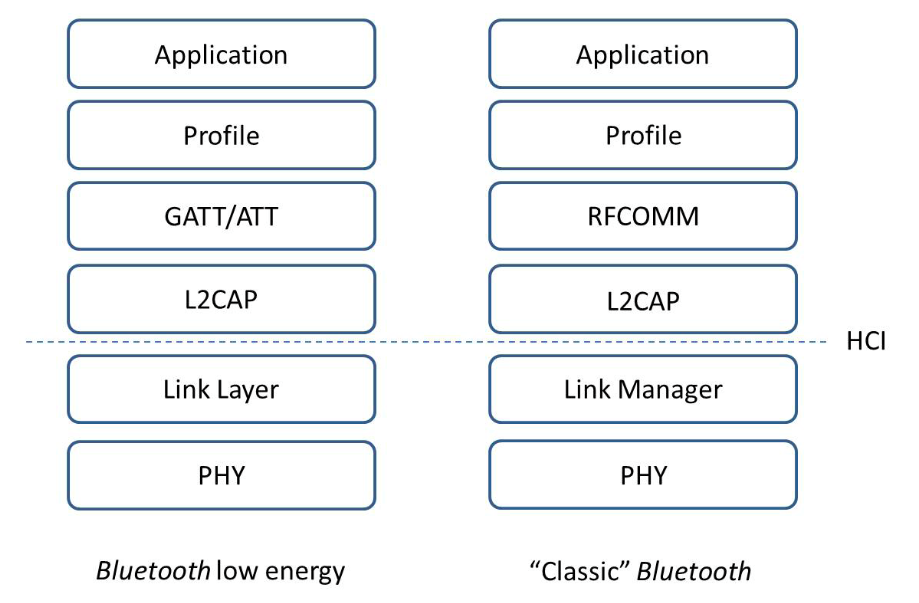
\includegraphics[width=0.7\textwidth]{images/ble/bluetooth_stack.png}
	\caption[Bluetooth Stack: \gls{bleLabel} und klassisches Bluetooth]{Bluetooth Stack: \gls{bleLabel} und klassisches Bluetooth (Quelle: \cite[][4]{ti_whitepaper_2015-05-08})}
%	\caption[The four-way handshake -- WPA]{\textit{The four-way handshake} -- \gls{wpaLabel} (Quelle: \cite[][151]{WrightCache201503})}
\end{figure}

% There are also differences at the profile layer. Bluetooth low energy profiles so far are all layered over GATT, using the GATT/ATT protocol to exchange data. In “classic” Bluetooth, profiles often define their own protocols. This is more flexible, but renders the implementation more complex and increases the amount of code that needs to run.

\section{Anwendungsfälle}
Mit \gls{bleLabel} wird der Markt für drahtlose Kommunikation stark erweitert.
Besonders wegen dem geringen Stromverbrauch und dem günstigen Preis, können viele alltägliche Geräte mit \gls{bleLabel} ausgestattet werden.
Die gleichzeitige stark wachsende Verbreitung von Smartphones die \gls{bleLabel} unterstützen, wecken zahlreiche neue interessante Datenaustäusche.

Auf der Bluetooth Website ist eine ausführliche Liste mit \gls{bleLabel} Geräten verfügbar.\footcite{Bluetooth_Smart_Devices_List_Bluetooth_Technology_Website_2015-05-14}
In folgenden Bereichen ist die Low Energy Variante bereits vertreten: Auto, Ortung im Verkauf, Unterhaltungstechnik, Gesundheit, Wellness, Mobiltelefone, Computer, Sport und modernen Haussteuerungen.

Folgende \cref{tab:usecases} soll das breite Spektrum an Anwendungsfälle aufzeigen:
\begin{table}[H]
	% style
	\small\sffamily\renewcommand{\arraystretch}{1.4}
	% caption
	\captionabove{\gls{bleLabel} Anwendungsfälle}
	\label{tab:usecases}
	\begin{tabular}{lp{0.35\linewidth}p{0.30\linewidth}}
		\toprule
		Kategorie & Geräte und Produkte & Anwendungsszenario (Beispiele)\\
		\midrule
		Auto & Schlüssel, Steuerung (Musik, GPS, etc.) & \textit{"'Find my car"'}-Systeme\\
		Ortung & Beacons & Ortsbasiertes Marketing mit Gutscheine\\
		Unterhaltungstechnik & Steuerung (TV, Musik, Bilder Wiedergabe) & Smartphonesteuerung für technische Gräte\\
		Gesundheit & Herzfrequenz, Blutdruck, Atemüberwachung, Waage, Zahnbürste & Überwachung von Gesundheitsmerkmalen (verschlüsselt)\\
		Computer, Mobiltelefone & Datenaustausch, Steuerung, Tastaturen & Überwachung und Steuerungen anderer Geräte\\
		Sport & Auswertung & Messung von Bewegung\\
		Haussteuerungen & Lampe, Garagentoor, Bewässerung, Smartwatch, Stylus,... & Technische Geräte starten bei Zugang eines Zimmer.\\
		\bottomrule
	\end{tabular}
\end{table}

Nebst diesen genannten Geräte gibt es unzählige weitere Einsatzmöglichkeiten für \gls{bleLabel}.
Viele der zukünftigen Geräte, werden einen kabellosen und standardisierten Datenaustausch für Steuer- und Analysezwecken nutzen können.
\footcite[][3,5]{ti_whitepaper_2015-05-08}

%So far, Bluetooth Smart has seen good adoption in the sports and fitness space. It also has great promise in medical and healthcare, in novel new use-cases such as proximity tags, beacons, computer peripherals and remote user interfaces. In recent months we have seen the rise of a new breed of “connected” devices based on Bluetooth Smart – including for home automation and smart metering, a raft of smart watches, proximity tags, activity monitoring and toothbrushes.

%The Bluetooth market has changed dramatically in the past three to four years. The technology has come a long way from being the wireless headset technology to leading the charge to connect innovative fitness monitors, door locks, credit cards, sports equipment, automobiles, gas sensors, light bulbs and a host of other applications. 



